\documentclass{article} % For LaTeX2e
\usepackage{nips15submit_e,times}
\usepackage{hyperref}
\usepackage{url}
%\documentstyle[nips14submit_09,times,art10]{article} % For LaTeX 2.09

\usepackage{amsfonts}
\usepackage{float}
\usepackage{boxedminipage}
\usepackage{multirow}
\usepackage{pbox}
\usepackage{graphicx}

\newfloat{Algorithm}{hbtp}{lop}[section]
\newcommand{\etal}{{\it et al.}}
\newcommand{\eps}{\epsilon}
\newcommand{\veps}{\varepsilon}
\newcommand{\kmpp}{{\tt $k$-means++seed}}
\newcommand{\ds}{{\tt $D^2$-seeding}}
\newcommand{\kmpar}{{\tt $k$-means$||$}}

\title{Fast Parallel Initialisation for $k$-means \\
\textcolor{red}{(Supplementary Material)}
}

%\author{
%Dipankar Das\\
%Intel Labs Bangalore\\
%\texttt{dipankar.das@intel.com} \\
%\And
%Jatin Garg \\
%IIT Delhi \\
%\texttt{cs1110223@cse.iitd.ac.in} \\
%\AND
%Sachin Goel \\
%IIT Delhi \\
%\texttt{cs1110249@cse.iitd.ac.in} \\
%\And
%Ragesh Jaiswal\thanks{Thanks to funding agencies.} \\\\
%IIT Delhi \\
%\texttt{rjaiswal@cse.iitd.ac.in} \\
%\And
%Sandeep Sen \\
%IIT Delhi \\
%\texttt{ssen@cse.iitd.ac.in}
%}

% The \author macro works with any number of authors. There are two commands
% used to separate the names and addresses of multiple authors: \And and \AND.
%
% Using \And between authors leaves it to \LaTeX{} to determine where to break
% the lines. Using \AND forces a linebreak at that point. So, if \LaTeX{}
% puts 3 of 4 authors names on the first line, and the last on the second
% line, try using \AND instead of \And before the third author name.

\newcommand{\fix}{\marginpar{FIX}}
\newcommand{\new}{\marginpar{NEW}}

%\nipsfinalcopy % Uncomment for camera-ready version

\begin{document}


\maketitle

%\begin{abstract}
%We provide a fast data-parallel initialization routine for $k$-means algorithm. 
The algorithm is based on sampling techniques that are easy to implement and parallelize. 
These parallel algorithms are implemented on a dual-socket Intel\textregistered Xeon\textregistered E5-2680v2. 
Empirical evaluations on large real and synthetic datasets demonstrates the practical utility of our techniques.
%\end{abstract}


\section{Fine grained analysis of {\tt $D^2$-seeding} w.r.t. parameter $N$}
We do a finer grained analysis of our algorithm's behaviour with respect to the parameter $N$.
The following table gives the mean value of the cost taken over $10$ runs.

\begin{table}[h]
\centering
\begin{tabular}{| l | c | c | c | c | c | c |}
\hline
 $\mathbf{N}$ & \pbox{2cm}{{\bf MNIST} \\\tiny($\times 10^{10}$)} & \pbox{2cm}{{\bf CIFAR} \\ \tiny{($\times 10^{10}$)}} & \pbox{2cm}{{\bf 3D} \\ \tiny{($\times 10^6$)}} & \pbox{2cm}{{\bf Birch1} \\ \tiny{($\times 10^{12}$)}} & \pbox{2cm}{{\bf Birch2} \\\tiny{($\times 10^{10}$)}} & \pbox{2cm}{{\bf Birch3} \\ \tiny{($\times 10^{12}$)}} \\
\hline \hline
$k$ & $31.98$	& $82.27$ & $17.22$ & $140.97$ & $72.51$ & $50.37$\\ 
\hline
$2k$ & $22.65$ & $57.68$ & $14.61$ & $131.82$ & $54.72$ & $47.92$\\ 
\hline
$5k$ & $21.42$ & $54.81$ & $12.90$ & $121.09$ & $51.53$ & $45.60$\\ 
\hline
$10k$ & $20.99$ & $53.05$ & $10.97$ & $122.42$ & $50.50$ & $45.49$\\ 
\hline
$15k$ & $21.33$ & $54.30$ & $11.46$ & $120.21$ & $49.29$ & $45.52$\\ 
\hline
$20k$ & $21.42$ & $52.86$ & $11.68$ & $121.53$ & $49.98$ & $44.59$\\ 
\hline
$30k$ & $21.11$ & $53.84$ & $10.87$ & $121.08$ & $50.39$ & $44.95$\\ 
\hline
$40k$ & $21.56$ & $53.36$ & $12.45$ & $120.29$ & $50.27$ & $44.79$\\ 
\hline
$50k$ & $21.20$ & $53.60$ & $11.32$ & $121.13$ & $49.52$ & $45.05$\\ 
\hline
$60k$ & $21.18$ & $52.90$ & $11.66$ & $119.77$ & $49.87$ & $44.61$\\ 
\hline
$70k$ & $20.99$ & $53.08$ & $11.31$ & $123.27$ & $49.17$ & $44.90$\\ 
\hline
$80k$ & $21.13$ & $53.68$ & $11.16$ & $121.38$ & $50.02$ & $46.02$\\ 
\hline
$90k$ & $21.08$ & $52.67$ & $11.64$ & $121.20$ & $50.84$ & $45.12$\\ 
\hline
$100k$ & $21.17$ & $52.80$ & $13.56$ & $121.93$ & $50.30$ & $45.12$\\ 
\hline
\end{tabular}
\caption{This table gives the cost of the solution produced by our seeding algorithm as a function of the input parameter $N$.}
\label{table:s1}
\end{table}

Figure~\ref{fig:s1} gives a plot for the above results. It is clear from the results that the improvement in cost obtained by increase of $N$ tends to diminish after $N = 10k$.


\begin{figure}
\centering
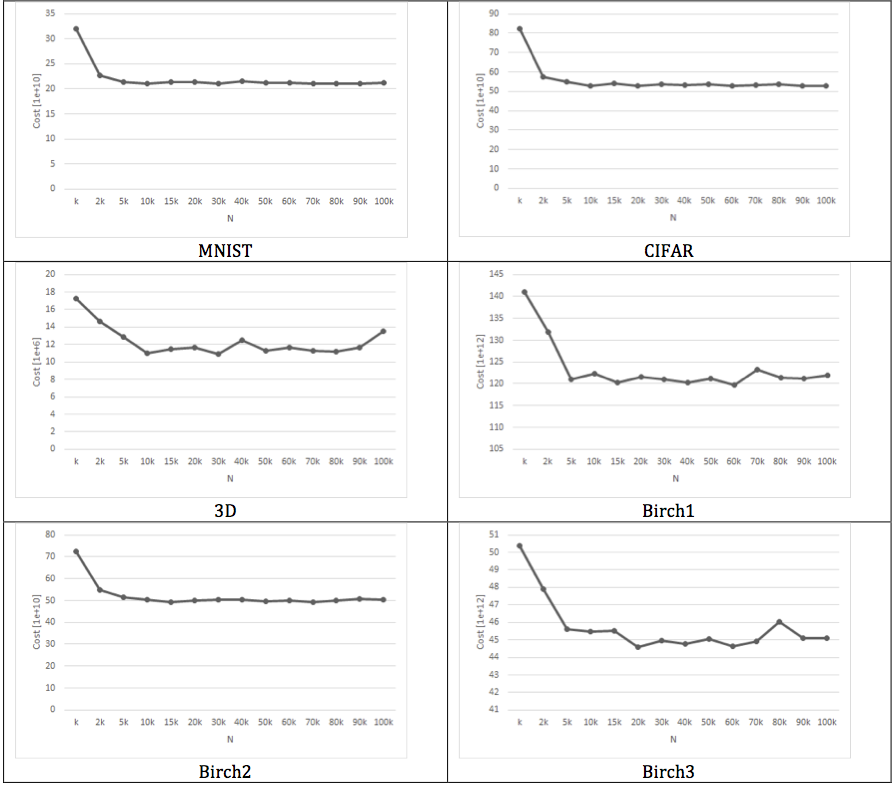
\includegraphics[scale=1]{Plots/N-plots}
\caption{Plot of cost with respect to $N$ for \ds\ algorithm.}
\label{fig:s1}
\end{figure}










\section{Comparing parallel seeding algorithms with parallel Lloyds with random seeding}
In the main writeup, we have given the cost/time comparison of parallel versions of various seeding algorithms.
Here, we add the cost/time values of the parallel version of the Lloyds algorithm with random seeding.
This is to show that seeding algorithms indeed do give cost/time advantages.
This is just to make sure that the quest for good ``seeding" algorithms are well motivated. 
The pseudocode for the parallel version of Lloyds algorithm is given in Algorithm~\ref{alg:s1}.

\begin{table}[H]
\centering
\begin{tabular}{| l | c | c | c || c | c || c | c |}
\hline
& & \multicolumn{2}{ c |}{{\bf MNIST}} & \multicolumn{2}{ c |}{{\bf CIFAR}} & \multicolumn{2}{ c |}{{\bf 3D}} \\ \cline{3-8}
{\bf Algorithm} & & \pbox{1cm}{Cost\\\tiny{($\times 10^{10}$)}} & \pbox{1cm}{Time\\ \tiny(in sec.)} & \pbox{1cm}{Cost\\\tiny{($\times 10^{10}$)}} & \pbox{1cm}{Time\\ \tiny(in sec.)} & \pbox{1cm}{Cost\\\tiny{($\times 10^6$)}} & \pbox{1cm}{Time\\ \tiny(in sec.)}\\
\hline \hline
\multirow{2}{*}{\pbox{3cm}{\small{Parallel Lloyds with} \\\small{random seed}}} & mean & 
$31.97$ & $9.75$ & $78.19$ & $32.48$ & $40.75$ & $4.02$\\ \cline{2-8}
& \small{sd} & ${\scriptstyle 1.27}$ & ${\scriptstyle 4.95}$ & ${\scriptstyle 6.11}$ & ${\scriptstyle 9.55}$ & ${\scriptstyle 23.70}$ & ${\scriptstyle 0.98}$\\
\hline \hline 
%
\multirow{2}{*}{\small{\tt Par-$k$-means++}} & mean & 
$32.42$ & $1.91$ & $80.45$ & $5.68$ & $17.82$ & $0.25$\\ \cline{2-8}
& \small{sd} & ${\scriptstyle 1.16}$ & ${\scriptstyle 0.51}$ & ${\scriptstyle 6.43}$ & ${\scriptstyle 0.47}$ & ${\scriptstyle 6.36}$ & ${\scriptstyle 0.03}$\\
\hline \hline 
%
\multirow{2}{*}{\pbox{5cm}{\small{\tt $k$-means$||$} \\ \tiny{($\ell=2k$, $r=5$)}}} & mean & 
$31.21$ & $10.68$ & $68.55$ & $34.29$ & $15.72$ & $2.92$\\ \cline{2-8}
& \small{sd} & ${\scriptstyle 1.02}$ & ${\scriptstyle 1.28}$ & ${\scriptstyle 2.89}$ & ${\scriptstyle 3.51}$ & ${\scriptstyle 5.06}$ & ${\scriptstyle 0.48}$\\
\hline \hline 
%
\multirow{2}{*}{\pbox{5cm}{\small{\tt Par-$D^2$-Seeding} \\ \tiny($N=10k$)}} & mean & 
$21.23$ & $2.26$ & $53.80$ & $6.72$ & $11.98$ & $0.27$\\ \cline{2-8}
& \small{sd} & ${\scriptstyle 0.49}$ & ${\scriptstyle 0.60}$ & ${\scriptstyle 1.33}$ & ${\scriptstyle 0.77}$ & ${\scriptstyle 2.02}$ & ${\scriptstyle 0.06}$\\
\hline
\end{tabular}
%\newline
%\vspace*{0.2cm}
%\newline
\bigskip
\vspace*{0.05cm}
\noindent
\begin{tabular}{| l | c | c | c || c | c || c | c |}
\hline
& & \multicolumn{2}{ c |}{{\bf Birch1}} & \multicolumn{2}{ c |}{{\bf Birch2}} & \multicolumn{2}{ c |}{{\bf Birch3}} \\ \cline{3-8}
{\bf Algorithm} & & \pbox{1cm}{Cost\\\tiny{($\times 10^{12}$)}} & \pbox{1cm}{Time\\ \tiny(in sec.)} & \pbox{1cm}{Cost\\\tiny{($\times 10^{10}$)}} & \pbox{1cm}{Time\\ \tiny(in sec.)} & \pbox{1cm}{Cost\\\tiny{($\times 10^{12}$)}} & \pbox{1cm}{Time\\ \tiny(in sec.)}\\
\hline \hline
\multirow{2}{*}{\pbox{3cm}{\small{Parallel Lloyds with} \\\small{random seed}}} & mean & 
$296.02$ & $21.95$ & $788.84$ & $9.80$ & $168.08$ & $28.24$\\ \cline{2-8}
& \small{sd} & ${\scriptstyle 25.04}$ & ${\scriptstyle 6.07}$ & ${\scriptstyle 233.23}$ & ${\scriptstyle 4.30}$ & ${\scriptstyle 37.34}$ & ${\scriptstyle 8.49}$\\
\hline \hline 
%
\multirow{2}{*}{\small{\tt Par-$k$-means++}} & mean & 
$189.54$ & $27.39$ & $165.16$ & $26.83$ & $67.78$ & $25.55$\\ \cline{2-8}
& \small{sd} & ${\scriptstyle 8.76}$ & ${\scriptstyle 2.33}$ & ${\scriptstyle 21.25}$ & ${\scriptstyle 2.27}$ & ${\scriptstyle 4.72}$ & ${\scriptstyle 3.24}$\\
\hline \hline 
%
\multirow{2}{*}{\pbox{5cm}{\small{\tt $k$-means$||$} \\ \tiny{($\ell=2k$, $r=5$)}}} & mean & 
$190.09$ & $9.93$ & $156.26$ & $10.15$ & $67.73$ & $10.21$\\ \cline{2-8}
& \small{sd} & ${\scriptstyle 10.86}$ & ${\scriptstyle 0.65}$ & ${\scriptstyle 20.28}$ & ${\scriptstyle 0.72}$ & ${\scriptstyle 3.43}$ & ${\scriptstyle 0.76}$\\
\hline \hline 
%
\multirow{2}{*}{\pbox{5cm}{\small{\tt Par-$D^2$-Seeding} \\ \tiny{($N=10k$)}}} & mean & 
$120.63$ & $37.16$ & $50.40$ & $36.51$ & $45.66$ & $38.50$\\ \cline{2-8}
& \small{sd} & ${\scriptstyle 8.76}$ & ${\scriptstyle 2.33}$ & ${\scriptstyle 1.84}$ & ${\scriptstyle 1.35}$ & ${\scriptstyle 1.09}$ & ${\scriptstyle 1.52}$\\
\hline
\end{tabular}
\caption{Running time and cost for parallel algorithms. The number of machine threads used is $M = 40$.}
\label{table:s2}
\end{table}


\begin{center}
\begin{Algorithm}[ht]
\begin{boxedminipage}{5.6in}
{\tt Parallel-lloyds($X, k, C$)}

\hspace{0.1in} (1) Repeat until convergence:

\hspace{0.3in} (a) Forall $1 \leq j \leq k$, $P[j] \leftarrow \bar{0}$, $numPoints[j] \leftarrow 0$.

\hspace{0.3in} (a) {\bf Parallel-for} $i \leftarrow $ $1$ to $|X|$:

\hspace{0.5in} (i) $j \leftarrow \arg\min_{l} \left\{ ||X[j] - C[l]||^2 \right\}$.

\hspace{0.5in} (ii) $P[j] \leftarrow P[j] + X[i]$; $numPoints[j] \leftarrow numPoints[j] + 1$.

\hspace{0.3in} (b) {\bf For} $i \leftarrow 1$ to $k$

\hspace{0.5in} (i) $C[i] \leftarrow \frac{P[i]}{numPoints[i]}$.

\hspace{0.1in} (2) Return $C$.
 \end{boxedminipage}
\caption{The parallel version of the Lloyds algorithm.}
\label{alg:s1}
\end{Algorithm}
\end{center}












\section{Comparing \kmpp, \kmpar,  and \ds}
All three algorithms, namely \kmpp, \kmpar, and \ds\ are sampling based algorithms with small differences.
It is important to understand these subtle differences between these algorithms.
\kmpp\ samples $k$ points in $k$ sequential steps where there is a clear forward dependency. 
The sampling distribution of the $i^{th}$ step depends on the centers chosen in the previous $(i-1)$ steps.
This forward dependency restricts parallelization since there is a $k$ size sequential component.
The \kmpar\ algorithm was designed precisely to avoid this sequential component. 
The main observation made was that if in each step, we sample more than one point independently then the sampled centers over even smaller number of iterations behave well.
So, if we sample roughly $\ell = 2k$ points independently in each iteration over as small as $r=5$ iterations, then the sampled points are nice with respect to the cost. 
However, the benefits (in terms of cost) of sampling points in a sequence as in \kmpp\ is compromised a bit.
On the other hand, since the sequential component has been reduced, the algorithm allows faster parallel versions.
This is the reason why the running time of \kmpar\ is consistently better than the other algorithms when $k$ is large (for Birch datasets $k$ is $100$).
The \ds\ algorithm, takes a slightly different approach with the main goal of obtaining solutions with smaller cost. 
It again picks centers in $k$ sequential steps as in the \kmpp\ algorithm.
However, it tries to pick a ``better" center in each step. 
It does so by independently sampling lots of points in each step. 
It then clusters these independently sampled points into $k$ clusters, picks the largest cluster, and then takes the centroid of the largest cluster.

The following hypothetical dataset highlights the difference between these three algorithms.
We note that on this hypothetical 1-dimensional dataset, the \kmpp\ and \ds\ algorithms give the optimal result whereas the \kmpar algorithm gives an arbitrarily bad result. 
Consider a large $k$ (say $k = 100$).
There are $2^{k}$ points co-located at origin, $10k$ point co-located at $1$, $10k$ points co-located at $k$, $10k$ points co-located at $k^2$, ..., $10k$ points co-located at $k^{k-1}$.
Clearly, the optimal $k$-means cost for this dataset is $0$.
Now, both the \kmpp\ and \ds\ algorithms on this dataset will pick one center each from the $k$ different locations and hence give the optimal solution. 
However, note the behaviour of \kmpar\ with $\ell = 2k$ and $r=5$. The first center is chosen uniformly at random, so most likely this will be a point from the origin. 
Subsequently, it will pick roughly $2k$ points independently in the first iteration. 
Given the distribution of the points, most likely all the points will be picked from location $k^{k-1}$.
In the second iteration, most likely all the points will be chosen from the location $k^{k-2}$ and so on. 
So, at the end of $r << k$ iterations, points from a only few locations (out of $k$) have been sampled and due to this, an arbitrarily bad non-optimal solution is produced.


\end{document}
